\documentclass{article}

% Geometry stuff
\usepackage[head=24pt,a4paper,lmargin={2.5cm},rmargin={2.5cm},tmargin={2.5cm},
bmargin={2.5cm}]{geometry}

% Tables
\usepackage{tabularx}

% Images
\usepackage{graphicx}

% Fancyhdr
\usepackage{fancyhdr}

\fancyhead[LO,LE]{
\includegraphics[scale=0.2]{./fig/uppsla_university.png}}

\fancyhead[RO,RE]{Comparision of Assays}

\fancyhead[CO,CE]{\today}

\fancyfoot[R]{Elmar van Rijnswou}

\fancyfoot[L]{Maximilian Stiefel}

% For links
\usepackage{hyperref}

% For floating
\usepackage{float} 

% For special characters
\usepackage{textcomp}

\begin{document}
\pagestyle{fancy}

\section{Alexa Fluor\textregistered 647 dye}

\begin{figure}[H]
	\centering
	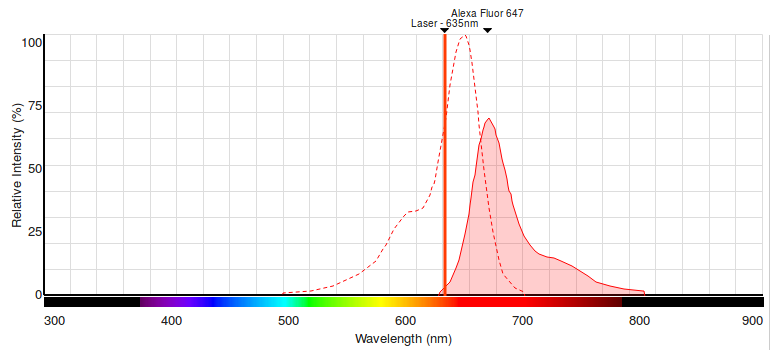
\includegraphics[width=0.8\textwidth]{./fig/spectrum_alexa_647_laser_635}
	\caption{Screenshot from the Thermo Fisher tool with the targeted laser.}
	\label{fig:alexa_647}
\end{figure}

\subsection{Overview of Coponents}
\begin{table}[H]
\centering
\begin{tabular}{lll}
\hline
\textbf{Product}                               & \textbf{Distributor} & \textbf{Price} \\\hline
Red Laser Diode 635 nm +/- 5 nm, 33 mA, 2.2 V  & Farnell         & 179.67 SEK     \\
Red Laser Diode 635 nm +/- 10 nm, 55 mA, 2.2 V & Aliexpress      & 2.5 \$ = 22.43 SEK \\
Photodiode BPW34                               & Farnell         & 7.48 SEK       \\
Longpass filter 675 nm                         & Edmund Optics   & 89 \$ = 798.33 SEK \\
Longpass filter 670 nm                         & Aliexpress      & 45.79 \$ = 402.49 SEK \\\hline
\end{tabular}
\caption{Materials needed for the Alexa Fluor® 647 dye.}
\label{tab:647}
\end{table}
\subsection{Laser Diode}
A good laser diode is available at Farnell:\\
\href{http://se.farnell.com/laser-components/2008352/laser-diode-635nm/dp/1272657?ost=laser+635+nm&categoryId=700000006112&searchView=table&iscrfnonsku=false}{http://se.farnell.com/laser-components/2008352/laser-diode-635nm/...}\\
Cheaper diodes are available from China:\\
\href{https://www.aliexpress.com/item/10-pcs-5mW-635nm-Orange-Red-TO18-5-6mm-N-type-Laser-Diode-LD-SANYO-DL/32622824538.html?spm=2114.01010208.3.322.KNKdbx&ws_ab_test=searchweb0_0,searchweb201602_3_10065_10068_10136_10137_10138_10060_10062_10141_10056_10055_10054_122_10059_10099_10103_10102_10096_10052_10053_10050_10107_10142_10051_10143_10084_10083_10080_10082_10081_10110_10111_10112_10113_10114_10078_10079_10073_10070_10123_10124,searchweb201603_2,afswitch_1,ppcSwitch_4,single_sort_0_default&btsid=b98573dc-6228-4b35-ad77-02e75b3fe435&algo_expid=3174f530-2df6-46b1-87c5-c36e2f9f58b0-38&algo_pvid=3174f530-2df6-46b1-87c5-c36e2f9f58b0}{https://www.aliexpress.com/item/10-pcs-5mW-635nm-Orange-Red-TO18-5-6mm-N-type-Laser-Diode-LD-SANYO-DL..}
\subsection{Photodiode}
The BPW34 is cheaply available at Farnell:\\
\href{http://se.farnell.com/vishay/bpw34/photodiode-2na-900nm-rectangular/dp/1045425}{http://se.farnell.com/vishay/bpw34/photodiode-2na-900nm-rectangular/dp/1045425}\\
One has to watch out as not all BPW34s have the same spectral sensitivity. This diode is also available cheaper in China.  
\subsection{Filter}
The filter can be obtained from Edmund Optics:\\
\href{https://www.edmundoptics.com/optics/optical-filters/longpass-edge-filters/longpass-filters/64621/}{https://www.edmundoptics.com/optics/optical-filters/longpass-edge-filters/longpass-filters/64621/}\\
Similar filters can be found in China:\\
\href{https://www.aliexpress.com/item/Diameter-60mm-HB670-IR-Band-Pass-Filter-Long-Wavelength-Band-Pass-Filter/32766997403.html?spm=2114.01010208.3.10.iVA9gb&ws_ab_test=searchweb0_0,searchweb201602_3_10065_10068_10136_10137_10138_10060_10062_10141_10056_10055_10054_122_10059_10099_10103_10102_10096_10052_10053_10050_10107_10142_10051_10143_10084_10083_10080_10082_10081_10110_10111_10112_10113_10114_10078_10079_10073_10070_10123_10124,searchweb201603_2,afswitch_1,ppcSwitch_4,single_sort_0_default&btsid=882bb4cb-2a55-4d1b-8d9b-0348a7b8ec5f&algo_expid=ee21d12d-5045-4fab-93e1-0a0a214c0df0-1&algo_pvid=ee21d12d-5045-4fab-93e1-0a0a214c0df0}{https://www.aliexpress.com/item/Diameter-60mm-HB670-IR-Band-Pass-Filter-Long-Wavelength-Band-Pass-Filter/...}
\begin{figure}[H]
	\centering
	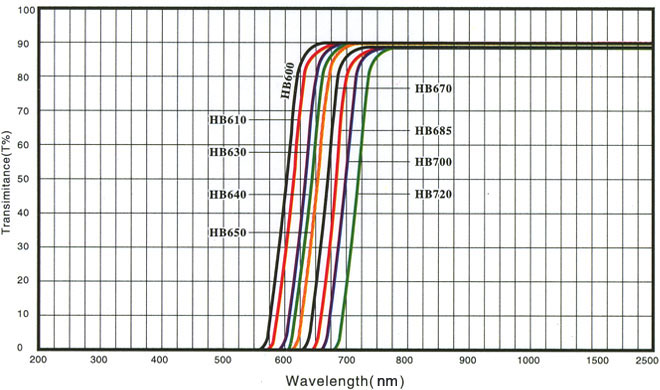
\includegraphics[width=0.8\textwidth]{./fig/spectra_filter_china}
	\caption{Chinese filters available from this distributer.}
	\label{fig:chines_filter}
\end{figure}
Before ordering we definitely have to talk to Uwe to double check if this filter works. There is a huge variety of available filters. Both filters are usable for multiple devices as one can cut them. Both filters are circle shaped and have a diametel of 12.5 mm.  

\section{Qdot\textregistered 800 streptavidin conjugate}

\begin{figure}[H]
	\centering
	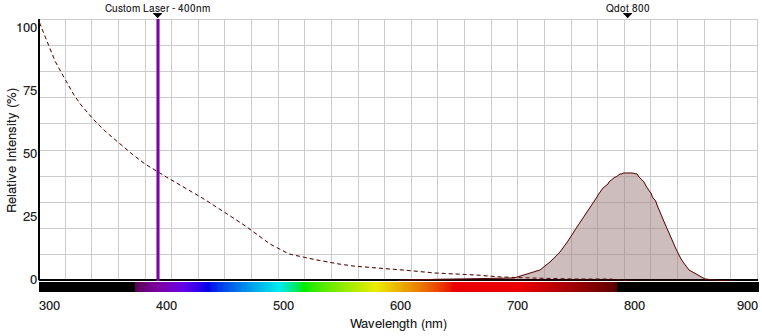
\includegraphics[width=0.8\textwidth]{./fig/spectrum_qdots_800_400}
	\caption{Screenshot from the Thermo Fisher tool with 400 nm laser. I reality this might be a UV LED.}
	\label{fig:qdots_800_400}
\end{figure}

\begin{figure}[H]
	\centering
	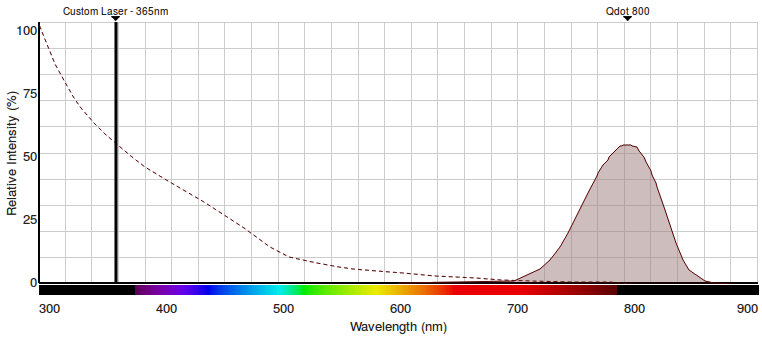
\includegraphics[width=0.8\textwidth]{./fig/spectrum_qdots_800_365}
	\caption{Screenshot from the Thermo Fisher tool with 365 nm laser. I reality this might be a Blacklight LED.}
	\label{fig:qdots_800_400}
\end{figure}

\subsection{Overview of Coponents}
\begin{table}[H]
\centering
\begin{tabular}{lll}
\hline
\textbf{Product}                               	& \textbf{Distributor} 	& \textbf{Price} \\\hline
UV LED 400 nm, 20 mA, 3.7 V			& Farnell		& 43.22 SEK	\\
UV LED 400 nm, 20 mA, 3 V			& Aliexpress		& 0.05 \$ = 0.45 SEK \\
UV LED 365 nm, 30 mA, 3.2 V			& Ebay			& 5 EUR = 47.8 SEK \\
Photodiode BPW34                              	& Farnell         	& 7.48 SEK       \\
Photodiode BPW34				& Aliexpress		& 0.281 \$ = 2.52 SEK \\
Photodiode BPW34FS				& Farnell		& 8.63 SEK \\\hline
\end{tabular}
\caption{Materials needed for the Alexa Fluor® 647 dye.}
\label{tab:647}
\end{table}

\subsection{LEDs}
Two different types of LEDs are possible. Either UV LEDs, which are quite cheap in China:\\
\href{https://www.aliexpress.com/item/100PCS-Purple-Color-5mm-Transparent-Water-ClearRound-Super-Bright-UV-LED-DIODE/32266780769.html?spm=2114.01010208.3.12.tra0j7&ws_ab_test=searchweb0_0,searchweb201602_3_10065_10068_10136_10137_10138_10060_10062_10141_10056_10055_10054_122_10059_10099_10103_10102_10096_10052_10053_10050_10107_10142_10051_10143_10084_10083_10080_10082_10081_10110_10111_10112_10113_10114_10078_10079_10073_10070_10123_10124-10111,searchweb201603_2,afswitch_1,ppcSwitch_5,single_sort_0_default&btsid=93ee4e21-8cbb-4573-8c94-fde0f528a3a4&algo_expid=a530b458-dbb3-4e8e-9b05-e6f5bf8dd6c4-1&algo_pvid=a530b458-dbb3-4e8e-9b05-e6f5bf8dd6c4}{https://www.aliexpress.com/item/100PCS-Purple-Color-5mm-Transparent-Water-ClearRound-Super-Bright-UV-LED-DIODE...}\\
Or quite expensive in Sweden:
\href{http://se.farnell.com/bivar/led3-uv-400-30/uv-led-3mm-30deg/dp/1057107}{http://se.farnell.com/bivar/led3-uv-400-30/uv-led-3mm-30deg/dp/1057107}\\
The other option, which is the better one, from my POV, are blacklight LEDs. Those are not really easily available. But there are some from Italy:
\href{http://www.ebay.de/itm/365nm-5-LED-UV-5mm-ULTRAVIOLETTI-ONDA-KURZ-ZWECKE-MEDICI-ULTRAVIOLETTE-STRAHLUNG-/121843052978?hash=item1c5e6971b2:m:mVQ-u99Iola62PpsoNnF26g}{http://www.ebay.de/itm/365nm-5-LED-UV-5mm-ULTRAVIOLETTI-ONDA-KURZ-ZWECKE-MEDICI-ULTRAVIOLETTE-STRAHLUNG-/121843052978?hash=item1c5e6971b2:m:mVQ-u99Iola62PpsoNnF26g}

\subsection{Photodiode}
The idea is to use a photodiode without any filter in this case. The filter is the most expensive part of the whole system. In the datasheet of the BPW34 one can read, that the diode works from \textbf{430 nm to 1100 nm}. This means, that possibly UV light with 400 nm or even 365 nm will not be received by this diode. We have to discuss this with Uwe or maybe even try it out. Datasheet of the BPW34:\\
\href{http://www.farnell.com/datasheets/2046123.pdf}{http://www.farnell.com/datasheets/2046123.pdf}\\
This photodiode is available cheaper from various sources e.g.:\\
\href{https://www.aliexpress.com/item/Smart-Electronics-10pcs-lot-BPW34-Photodiode/32711869804.html?spm=2114.01010208.3.37.kEUjrU&ws_ab_test=searchweb0_0,searchweb201602_3_10065_10068_10136_10137_10138_10060_10062_10141_10056_10055_10054_122_10059_10099_10103_10102_10096_10052_10053_10050_10107_10142_10051_10143_10084_10083_10080_10082_10081_10110_10111_10112_10113_10114_10078_10079_10073_10070_10123_10124,searchweb201603_2,afswitch_1,ppcSwitch_5,single_sort_0_default&btsid=7135d04f-8309-410c-a0c5-9b6acfaec429&algo_expid=395c0e88-612b-46b8-bc3a-0ed4465fb75e-4&algo_pvid=395c0e88-612b-46b8-bc3a-0ed4465fb75e}{https://www.aliexpress.com/item/Smart-Electronics-10pcs-lot-BPW34-Photodiode/...}\\
Another option is maybe the BPW34FS, which is equiped with a "daylight filter", which results another spectral range of sensitivity (\textbf{780 nm to 1100 nm}):
\href{http://se.farnell.com/osram/bpw34fs/photodiode-ir-filter-950nm-60deg/dp/1212747}{http://se.farnell.com/osram/bpw34fs/photodiode-ir-filter-950nm-60deg/dp/1212747}


\end{document}
